%-----------------------------------------------------------------------------%
\chapter{\babDua}
%-----------------------------------------------------------------------------%

Pada bab ini, akan dijelaskan mengenai landasan teori yang menjadi dasar untuk memahami, menganalisis, dan menyelesaikan permasalahan yang menjadi fokus penelitian ini.

%-----------------------------------------------------------------------------%
\section{\cc}
%-----------------------------------------------------------------------------%
\cc, menurut definisi National Institute of Standards and Technology (NIST), merupakan suatu model komputasi yang menyediakan akses dan konfigurasi sumber daya komputasi seperti jaringan, server, penyimpanan, aplikasi, dan layanan secara on-demand, memungkinkan pelepasan yang cepat tanpa interaksi yang kompleks dengan penyedia layanan\cite{mell2009nist}. \cc\ bukanlah suatu teknologi spesifik, melainkan sebuah model yang menggambarkan operasional dan ekonomi untuk penyediaan serta penggunaan infrastruktur IT dan layanan terkait. Beberapa definisi cloud memiliki karakteristik umum yang sama, seperti \f{pay-per-use} (pembayaran sesuai dengan penggunaan), kapasitas yang elastis, layanan mandiri, dan abstraksi atau virtualisasi sumber daya\cite{Buyya_Broberg_Goscinski_2011}. NIST membagi model layanan cloud menjadi\cite{mell2009nist}:
\begin{enumerate}
	\item Software As A Service (SaaS)

	      Konsumen dapat memanfaatkan kemampuan dengan menggunakan aplikasi penyedia yang beroperasi di dalam infrastruktur cloud. Aplikasi tersebut dapat diakses dari berbagai perangkat klien melalui antarmuka klien yang ringan, seperti browser web (contohnya, email berbasis web), atau antarmuka program. Pengguna tidak perlu mengelola atau mengontrol infrastruktur cloud yang mendasarinya, termasuk jaringan, server, sistem operasi, penyimpanan, atau bahkan kemampuan aplikasi individual, kecuali mungkin pada pengaturan konfigurasi aplikasi khusus pengguna yang terbatas.


	\item Platform As A Service (PaaS)

	      Konsumen diberikan kemampuan untuk mendeploy aplikasi yang mereka buat atau peroleh ke infrastruktur cloud, menggunakan bahasa pemrograman, \f{library}, layanan, dan alat yang didukung oleh penyedia. Pengguna tidak perlu mengelola atau mengontrol infrastruktur cloud yang mendasarinya, termasuk jaringan, server, sistem operasi, atau penyimpanan. Meskipun begitu, pengguna tetap memiliki kendali atas aplikasi yang diimplementasikan dan mungkin dapat mengatur konfigurasi lingkungan hosting aplikasi.


	\item Infrastructure As A Service (IaaS)

	      Kemampuan yang diberikan kepada konsumen adalah untuk menyediakan sumber daya pemrosesan, penyimpanan, jaringan, dan sumber daya komputasi dasar lainnya di mana konsumen dapat mendeploy dan menjalankan perangkat lunak sembarang, yang dapat mencakup sistem operasi dan aplikasi. Konsumen tidak mengelola atau mengendalikan infrastruktur awan yang mendasari tetapi memiliki kendali atas sistem operasi, penyimpanan, dan aplikasi yang didistribusikan; dan mungkin kendali terbatas terhadap beberapa komponen jaringan tertentu (misalnya, firewall host).
\end{enumerate}


%-----------------------------------------------------------------------------%
\section{Apache CloudStack}
%-----------------------------------------------------------------------------%
\begin{figure}
	\centering
	
\includegraphics[width=0.70\textwidth]
	{assets/pics/apache_cloudstack_with_cloud_monkey.jpg}
	\caption{Logo Apache CloudStack}
	\label{fig:LogoApacheCloudStack}
\end{figure}
Apache CloudStack adalah perangkat lunak \oss\ yang dirancang untuk mendeploy dan mengelola jaringan besar mesin virtual, sebagai platform komputasi awan berbasis Infrastructure as a Service (IaaS) yang sangat tersedia dan dapat \f{scaleable}\cite{cloudstackabout}. Pada Gambar \ref{fig:LogoApacheCloudStack} adalah logo dari Apache Cloudstack. CloudStack digunakan oleh sejumlah penyedia layanan untuk menawarkan layanan cloud publik, dan oleh banyak perusahaan untuk menyediakan penawaran cloud \f{on-premise} (pribadi), atau sebagai bagian dari solusi cloud hybrid\cite{cloudstackabout}.

CloudStack adalah solusi siap pakai yang mencakup seluruh "stack" fitur yang paling diinginkan oleh organisasi dengan IaaS cloud: orkestrasi komputasi, Jaringan sebagai Layanan, manajemen pengguna dan akun, dan antarmuka Pengguna (UI) yang baik\cite{cloudstackabout}.

CloudStack saat ini mendukung hypervisor paling populer: VMware, KVM, Citrix XenServer, Xen Cloud Platform (XCP), Oracle VM server, dan Microsoft Hyper-V\cite{cloudstackabout}.

Pengguna dapat mengelola cloud mereka dengan antarmuka web yang mudah digunakan, alat \f{commandline}, dan/atau API RESTful yang lengkap. Selain itu, CloudStack menyediakan API yang kompatibel dengan AWS EC2 dan S3 untuk organisasi yang ingin mendeploy cloud secara hybrid\cite{cloudstackabout}.

CloudStack, yang awalnya dikembangkan oleh Cloud.com, diakuisisi oleh Citrix pada tahun 2011 dan diserahkan kepada Apache Software Foundation pada tahun 2012. Pengembangan saat ini diatur oleh Apache Foundation dengan kode yang tersedia di bawah lisensi Apache 2.0\cite{techtargetcloudstack}.


%-----------------------------------------------------------------------------%
\section{Hypervisor}
%-----------------------------------------------------------------------------%
Sebuah hypervisor adalah perangkat lunak atau perangkat keras yang digunakan untuk menciptakan dan mengelola mesin virtual. Juga dikenal sebagai \f{'Virtual Machine Monitor'} atau VMM, hypervisor memungkinkan satu server fisik menjalankan beberapa mesin virtual, mengatasi keterbatasan satu sistem operasi pada satu server. Hypervisor dapat berupa perangkat keras atau program, dan fungsinya adalah menciptakan, memonitor, dan mengelola mesin-mesin virtual\cite{MacPherson_2023}.

\begin{figure}
	\centering
	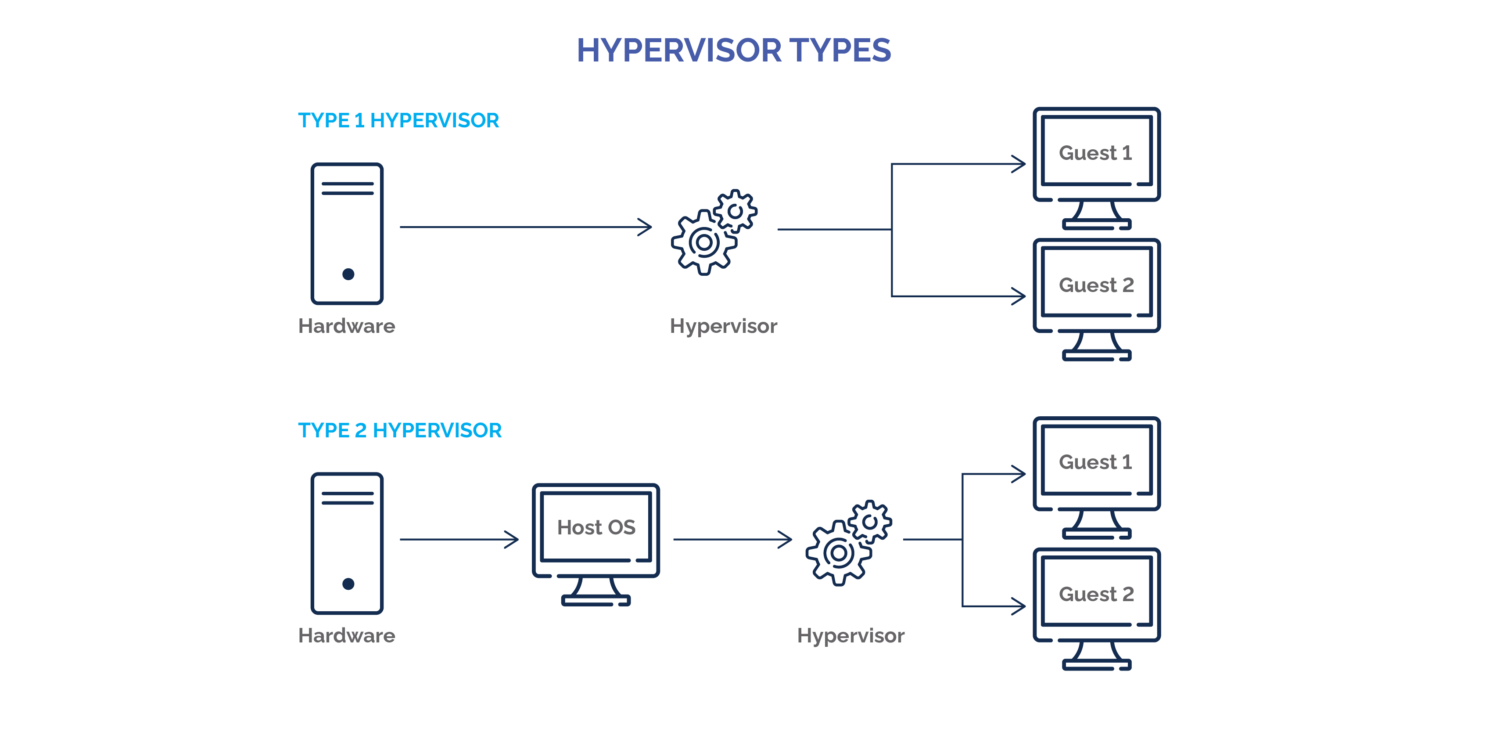
\includegraphics[width=1\textwidth]
	{assets/pics/type-1-hypervisor-vs-type-2.png}
	\caption{Hypervisor Type 1 vs Type 2}
	\label{fig:HypervisorType1vsType2}
\end{figure}

Pada Gambar \ref{fig:HypervisorType1vsType2} diperlihatkan diagram sederhana perbedaan daripada Hypervisor tipe 1 dan Hypervisor tipe 2. Hypervisor tipe 1 dan tipe 2 merupakan perangkat lunak yang digunakan untuk menjalankan satu atau lebih \vm\ (VM) pada satu mesin fisik. \vm\ adalah replika digital dari mesin fisik, menciptakan lingkungan komputasi terisolasi yang pengguna alami sebagai sepenuhnya independen dari perangkat keras yang mendasarinya\cite{hypervisor1vs2}. Hypervisor mengelola dan mengalokasikan sumber daya fisik ke VM dan berkomunikasi dengan perangkat keras di latar belakang. Hypervisor tipe 1 ditempatkan di atas server tanpa sistem operasi dan memiliki akses langsung ke sumber daya perangkat keras, sehingga dikenal juga sebagai \f{bare metal} hypervisor. Sebaliknya, hypervisor tipe 2 adalah aplikasi yang diinstal pada sistem operasi host dan juga dikenal sebagai \f{hosted} atau \f{embedded} hypervisor\cite{hypervisor1vs2}.


%-----------------------------------------------------------------------------%
\section{KVM \f{(Kernel-Based Virtual Machine)}}
%-----------------------------------------------------------------------------%

KVM (Kernel-based Virtual Machine) merupakan modul virtualisasi \oss\ dan gratis dalam kernel Linux yang memungkinkan kernel berfungsi sebagai hypervisor. KVM adalah hypervisor tipe 1 atau biasa juga disebut sebagai hypervisor \f{bare metal}. KVM memungkinkan mesin host menjalankan beberapa lingkungan virtual terisolasi yang disebut sebagai guest atau \vm\ (VM).KVM (Kernel-based Virtual Machine) merupakan modul virtualisasi sumber terbuka dan gratis dalam kernel Linux yang memungkinkan kernel berfungsi sebagai hypervisor. Ini adalah tipe-1 (bare-metal) hypervisor yang memungkinkan mesin host menjalankan beberapa lingkungan virtual terisolasi yang disebut sebagai guest atau mesin virtual (VM).

KVM telah disatukan ke dalam kernel Linux utama pada versi 2.6.20, yang dirilis pada 5 Februari 2007. Untuk dapat berjalan, KVM memerlukan prosesor dengan ekstensi virtualisasi perangkat keras, seperti Intel VT atau AMD-V. KVM menyediakan abstraksi perangkat tetapi tidak ada emulasi prosesor. Modul ini mengekspos antarmuka /dev/kvm, yang dapat digunakan oleh mode pengguna untuk menyiapkan ruang alamat VM guest.

KVM mendukung virtualisasi perangkat keras untuk berbagai sistem operasi guest, termasuk BSD, Solaris, Windows, Haiku, ReactOS, Plan 9, dan lainnya. Sebagai bagian dari kernel Linux, KVM langsung mengambil manfaat dari setiap fitur baru, perbaikan, dan kemajuan Linux tanpa perlu rekayasa tambahan.

Dalam pengaturan KVM, CPU virtual dari VM diimplementasikan sebagai thread (disebut "virtual CPU" atau vcpu) yang dijadwalkan oleh \f{Linux Kernel Scheduler}. KVM pada dasarnya adalah pengemudi untuk ekstensi virtualisasi processor. Setiap kali \f{Linux Scheduler} memilih tugas untuk dijalankan pada CPU fisik, dan tugas tersebut dikerjakan oleh CPU virtual dari VM, KVM "dihubungi" untuk memastikan bahwa yang sebenarnya berjalan di perangkat keras adalah program dari OS guest\cite{Abeni2020}.

\begin{figure}
	\centering
	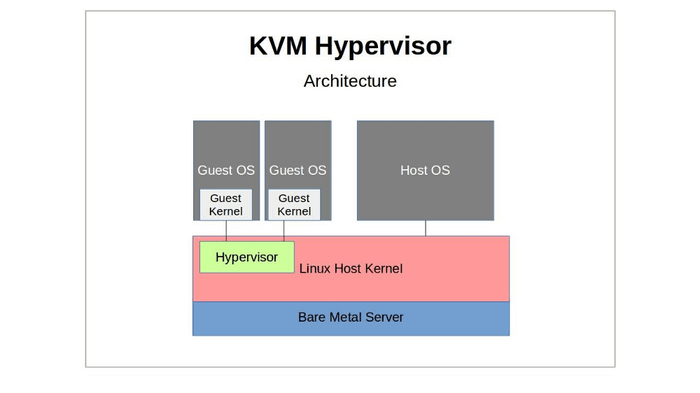
\includegraphics[width=1\textwidth]
	{assets/pics/xen-kvm.png}
	\caption{Arsitektur Hypervisor KVM}
	\label{fig:xen-kvm}
\end{figure}

Pada Gambar \ref{fig:xen-kvm} adalah struktur daripada hypervisor KVM. KVM berjalan langsung pada kernel linux host dan membagikan resourcenya kepada guest \vm, sedangkan sistem operasi host berjalan langsung diatas kernel host. Sistem operasi host dapat melakukan konfigurasi kepada \vm\ yang menggunakan hypervisor miliknya.

%-----------------------------------------------------------------------------%
\section{\f{Virtual Machine}}
%-----------------------------------------------------------------------------%

Virtual Machine (VM) adalah sebuah lingkungan komputasi yang dibuat secara virtual di dalam sebuah komputer fisik (host)\cite{Pradilla2016}. VM ini berfungsi seperti sebuah komputer independen yang dapat menjalankan sistem operasi dan aplikasi seperti komputer fisik biasa, tetapi semuanya berjalan dalam lingkungan virtual yang terisolasi di dalam host fisik. Setiap \vm\ (VM) menjalankan sistem operasi secara independen dan beroperasi terpisah dari VM lainnya, bahkan ketika semuanya berjalan pada host yang sama. Perangkat lunak yang dikenal sebagai hypervisor atau \vmm\ (VMM) memungkinkan kita untuk menjalankan berbagai sistem operasi yang berbeda secara bersamaan pada \vm\ yang berbeda. VM memiliki beberapa keunggulan dibandingkan dengan mesin fisik, termasuk kemampuan untuk menjalankan beberapa lingkungan sistem operasi pada satu komputer fisik, mendukung aplikasi \f{legacy}, dan menyediakan opsi pemulihan dalam situasi bencana. VM digunakan untuk berbagai keperluan, seperti \cc, pengujian sistem operasi baru, dan menjalankan beberapa aplikasi pada satu mesin fisik\cite{ibmWhatVirtualMachine}.

\begin{figure}
	\centering
	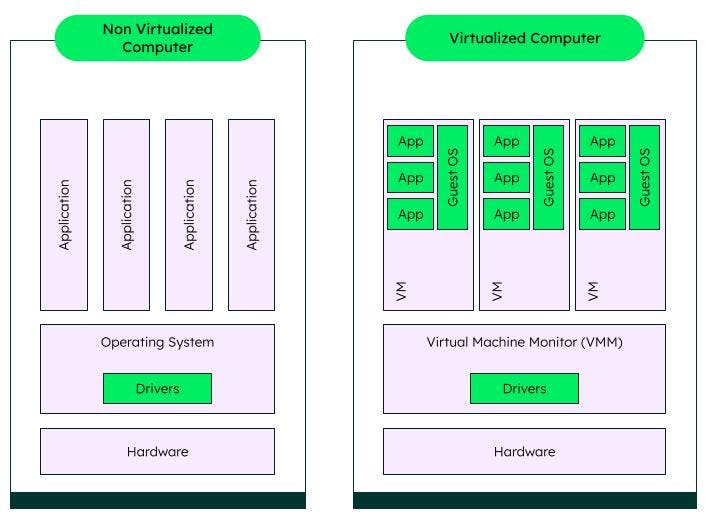
\includegraphics[width=1\textwidth]
	{assets/pics/vm-diagram.jpg}
	\caption{Perbedaan Komputasi Tanpa Virtualisasi dengan Virtualisasi}
	\label{fig:vm-diagram}
\end{figure}

Terdapat perbedaan dalam cara berjalan antara komputer tanpa virtualisasi (host) dan komputer yang divirtualisasi (guest) atau \vm. Pada Gambar 2.4, dapat diperlihatkan bahwa pada komputer tanpa virtualisasi, sistem operasinya berjalan langsung di atas perangkat keras, dengan driver yang berfungsi sebagai jembatan, sehingga aplikasi dapat berjalan langsung di atas sistem operasi tersebut. Di sisi lain, pada komputer yang divirtualisasi, sistem operasinya berjalan di atas VMM atau Virtual Machine Monitor, di mana satu VMM dapat menjalankan banyak sistem operasi guest.

%-----------------------------------------------------------------------------%
\section{\f{Advanced Encryption Standard} (AES)}
%-----------------------------------------------------------------------------%
\f{Advanced Encryption Standard} atau disingkat AES pertama kali diumumkan oleh NIST \f{(National Institute Of Standards and Technology)} pada tahun 2001 sebagai pengganti algoritma DES yang semakin mudah diretas. AES merupakan hasil dari kompetisi yang diadakan oleh NIST pada tahun 1997 yang dimenangkan oleh tim dari belgium yang memiliki nama asli Rijndael. Rijndael dikembangkan oleh dua orang kriptografer dari belgium bernama Joan Daemen dan Vincent Rijmen. AES dipublikasikan oleh NIST pada tahun 2001 dan tersebar secara efektif pada bulan May 2002 setelah disetujui oleh Menteri Perdagan Amerika, Donald Evans\cite{Kaffahemailencryptaes}.

AES merupakan metode enkripsi data dengan teknik enkripsi simetris, yang berarti menggunakan kunci yang sama untuk proses enkripsi dan dekripsi. Kunci pada AES tersedia dalam tiga varian ukuran, yakni 128 bit, 192 bit, dan 256 bit. Meskipun ukuran kuncinya bervariasi, ukuran blok data yang dienkripsi tetap sama, yaitu 128 bit. Ukuran blok mengacu pada cara data dienkripsi dengan memecah dan menyusunnya. Data disusun menjadi array 4x4 berukuran 16 byte, di mana setiap byte terdiri dari 8 bit, sehingga total setiap blok berjumlah 128 bit\cite{NistAes}.



%-----------------------------------------------------------------------------%
\section{\f{Cyclic Redundancy Check} (CRC)}
%-----------------------------------------------------------------------------%
\f{Cyclic Redundancy Check} (CRC) merupakan teknik yang digunakan untuk mendeteksi kesalahan dalam transmisi data digital. Teknik ini melibatkan penambahan kode pemeriksaan pada data untuk mengidentifikasi kesalahan yang mungkin terjadi selama proses transmisi. CRC didasarkan pada konsep pembagian polinomial, khususnya dengan menggunakan \f{Linear Feedback Shift Registers} (LFSRs).

\begin{enumerate}
	\item Gambaran Teknik CRC\cite{zhangLowComplexityCRC}:
	      \begin{itemize}
		      \item CRC digunakan untuk mendeteksi kesalahan dalam data digital, terutama pada aplikasi yang beroperasi dengan kecepatan tinggi.
		      \item CRC menggunakan \f{Linear Feedback Shift Registers} untuk deteksi kesalahan.
		      \item Teknik ini melibatkan pembagian biner untuk menghasilkan sisa (CRC) yang kemudian ditambahkan ke data sebagai pemeriksaan kesalahan di penerima.
	      \end{itemize}

	\item Prinsip CRC\cite{SrideviCRCDataRecovery}:
	      \begin{itemize}
		      \item Teknik CRC menambahkan kode pemeriksaan r-bit ke kode informasi k-bit, membentuk kode (n, k) dengan panjang n(k + r) bit.
		      \item Setiap kode (n, k) memiliki polinomial g(x) dengan kekuatan maksimum n-k=r terkait dengannya, dikenal sebagai polinomial yang dihasilkan dari kode CRC.
		      \item Kode CRC umumnya ditempatkan di akhir informasi untuk mendeteksi kesalahan selama transmisi.
		      \item Di sisi penerima, perhitungan CRC dilakukan pada informasi yang diterima untuk memeriksa kesalahan.
		      \item Implementasi seperti CRC-5, CRC-8, dan CRC-32 menunjukkan optimasi dan efisiensi yang spesifik untuk protokol dan sistem yang berbeda.
	      \end{itemize}
\end{enumerate}


%-----------------------------------------------------------------------------%
\section{virsh}
%-----------------------------------------------------------------------------%

virsh adalah \f{command line tool} yang merupakan bagian dari \f{library} libvirt dan secara utama digunakan untuk mengelola dan berinteraksi dengan teknologi virtualisasi pada sistem Linux, khususnya KVM (Kernel-based Virtual Machine) dan QEMU (Quick Emulator), dan mendukung hypervisor lainnya seperti Xen, LXC, OpenVZ, VirtualBox, dan VMware ESX\cite{libvirtLibvirtVirsh}.

Secara sederhana penggunaan virsh adalah seperti ini
\begin{center}
	\begin{verbatim}
		virsh [OPTION]... <command> <domain> [ARG]...
	\end{verbatim}
\end{center}

Pada command ini, domain adalah ID domain numerik, atau nama domain, atau UUID domain; dan ARGS adalah opsi khusus dari command. Setiap command yang dimulai dengan \# dianggap sebagai komentar dan diabaikan oleh sistem, semua perintah yang tidak dikenali akan didiagnosis.

%-----------------------------------------------------------------------------%
\section{\f{Streaming SIMD Extensions}}
%-----------------------------------------------------------------------------%
Streaming SIMD Extensions (SSE) adalah instruksi yang dibawa oleh Intel pada tahun 1999 dengan prosesor Pentium III dengan tujuan untuk meningkatkan kinerja prosesor arsitektur x86. Awalnya dikenal sebagai Katmai New Instructions (KNI) selama pengembangan, SSE secara signifikan meningkatkan kemampuan pemrosesan multimedia dan grafis dibanding pendahulunya, MMX. SSE mencakup 70 instruksi baru yang dirancang untuk meningkatkan tugas seperti pengolahan gambar, video 3D, audio dan video streaming, serta pengenalan suara\cite{informitStreamingSIMD}.

Tidak seperti pendahulunya, MMX menggunakan unit floating-point standar yang sama, sedangkan SSE menggunakan unit terpisah dalam prosesor untuk perhitungan floating-point, yang memungkinkan pemrosesan yang lebih efisien. SSE mendukung operasi floating-point SIMD (Single Instruction Multiple Data) single precision, yang sangat penting untuk mengatasi bottleneck dalam pemrosesan grafis 3D. Teknologi ini memungkinkan satu instruksi untuk melakukan hingga empat operasi floating-point secara bersamaan, meningkatkan kecepatan dan efisiensi pemrosesan\cite{informitStreamingSIMD}.

Manfaat SSE yang utama terlihat dalam decoding MPEG2, format standar untuk video DVD, memungkinkan prosesor yang dilengkapi SSE untuk menangani decoding tersebut di perangkat lunak dengan kecepatan penuh tanpa perangkat keras tambahan. SSE juga meningkatkan penggunaan CPU dan kinerja perangkat lunak pengenalan suara, memberikan akurasi yang lebih tinggi dan waktu respons yang lebih cepat. Untuk sepenuhnya memanfaatkan kemampuan SSE, aplikasi harus diset secara khusus agar SSE-aware, sebuah fitur yang sekarang umum dalam banyak aplikasi grafis dan berhubungan dengan suara. SSE adalah perluasan dari MMX, yang berarti bahwa prosesor yang mendukung SSE juga kompatibel dengan instruksi MMX, hal ini memastikan \f{backward compatibility} dengan aplikasi yang mendukung MMX\cite{informitStreamingSIMD}.

SSE telah berkembang seiring waktu dengan versi seperti SSE2, SSE3, dan SSE4, masing-masing membawa fitur baru dan meningkatkan kemampuan pemrosesan secara keseluruhan. Ekstensi ini telah banyak diadopsi dalam pengembangan perangkat lunak, terutama dalam bidang di mana pemrosesan paralel sangat penting.

\subsection{SSE2}
SSE2 adalah perluasan dari kemampuan SIMD (Single Instruction, Multiple Data) yang awalnya diperkenalkan dengan set instruksi SSE (Streaming SIMD Extensions). Pertama kali diperkenalkan oleh Intel dengan prosesor Pentium 4\cite{SystemVAppBinaryInterfaceMichael}. Perbedaan utama dan peningkatan dalam SSE2 dibandingkan dengan pendahulunya SSE meliputi:

\begin{enumerate}
	\item Rentang Jenis Data yang Lebih Luas

	      SSE2 memperluas kemampuan SIMD untuk beroperasi pada data integer 64-bit dan data floating-point presisi ganda (SSE terutama berfokus pada operasi floating-point presisi tunggal).

	\item Peningkatan Set Instruksi

	      SSE2 menambahkan instruksi dan kemampuan baru, meningkatkan pengolahan dan manipulasi berbagai jenis data, termasuk integer terpak (packed integers) dan angka floating-point presisi ganda.

	\item Peningkatan Kinerja untuk Aplikasi Ilmiah dan Multimedia

	      Dengan menyediakan operasi pada tipe data yang lebih besar dan set operasi yang lebih luas, SSE2 meningkatkan efisiensi dan kinerja aplikasi yang berhubungan dengan perhitungan matematika kompleks, grafik 3D, pengkodean video, dan tugas multimedia lainnya.
\end{enumerate}

Penggabungan SSE2 dalam arsitektur AMD64 menyoroti pentingnya dalam komputasi modern, terutama untuk aplikasi yang memerlukan kinerja tinggi dalam pengolahan numerik dan multimedia. Dokumen ABI kemungkinan mengasumsikan keakraban dengan konsep-konsep ini, lebih berfokus pada detail implementasi dalam arsitektur AMD64 daripada menjelaskan perbedaan fundamental antara SSE dan SSE2\cite{SystemVAppBinaryInterfaceMichael}.

\subsection{SSE3}
SSE3 (Streaming SIMD Extensions 3) merupakan ekstensi dari set instruksi SSE2, yang mana memperluas teknologi SSE (Streaming SIMD Extensions) asli. Perbedaan antara SSE3 dengan SSE2 antara lain:

\begin{enumerate}
	\item 13 Set Instruksi Baru

	      SSE3 menambahkan tiga belas instruksi baru ke set instruksi SSE/SSE2 yang ada\cite{Hassaballah2008}.

	\item Dukungan untuk Model Eksekusi SIMD:

	      Dari 13 instruksi ini, sepuluh dirancang untuk mendukung model eksekusi SIMD (Single Instruction, Multiple Data). Model ini merupakan aspek penting dari komputasi paralel, di mana beberapa titik data diproses secara bersamaan menggunakan satu instruksi. Ini sangat bermanfaat untuk tugas-tugas seperti pengolahan grafis, perhitungan ilmiah, dan aplikasi multimedia, di mana operasi pada set data besar adalah hal yang umum\cite{Hassaballah2008}.

	\item Konversi Floating-Point ke Integer:

	      Salah satu instruksi SSE3 secara spesifik mempercepat pemrograman \f{x87-style}. Instruksi ini berfokus pada peningkatan efisiensi dalam mengkonversi nilai floating-point menjadi integer. Hal ini bisa sangat berguna dalam skenario di mana perhitungan melibatkan tipe data floating-point dan integer\cite{Hassaballah2008}.

	\item Akselerasi Sinkronisasi Thread:

	      Dua instruksi lain dalam set SSE3 ditujukan untuk meningkatkan sinkronisasi thread. Peningkatan ini sangat penting dalam aplikasi multi-thread, di mana pengelolaan eksekusi dan koordinasi beberapa thread adalah kunci untuk kinerja yang baik dan efisiensi\cite{Hassaballah2008}.
\end{enumerate}

Secara singkat, SSE3 memperluas kemampuan set instruksi SSE dan SSE2 dengan penekanan pada peningkatan eksekusi SIMD, konversi floating-point ke integer, serta sinkronisasi thread. Selain itu, SSE3 tetap mempertahankan kompatibilitas dengan jenis data dan lingkungan pemrograman yang sudah ada. Oleh karena itu, SSE3 menjadi alat yang sangat berguna bagi pengembang yang bekerja pada tugas komputasi berkinerja tinggi, terutama yang melibatkan pemrosesan paralel dan jenis data yang kompleks.

\subsection{SSSE3}
SSSE3 (Supplemental Streaming SIMD Extensions 3) adalah ekstensi dari set instruksi SSE3 yang diperkenalkan oleh Intel pada tahun 2006. SSSE3 menambahkan 32 instruksi baru ke set instruksi SSE3 yang ada, yang dirancang untuk meningkatkan kinerja pemrosesan SIMD (Single Instruction, Multiple Data) pada aplikasi yang memerlukan operasi vektorisasi dan paralel. Pembaruan dari SSSE3 antara lain:

\begin{enumerate}
	\item Dua belas instruksi yang melakukan operasi penambahan atau pengurangan horizontal.
	\item Enam instruksi yang mengevaluasi nilai absolut.
	\item Dua instruksi yang melakukan operasi perkalian-dan-penambahan dan mempercepat evaluasi \f{dot product}.
	\item Dua instruksi yang mempercepat operasi perkalian bilangan bulat dan menghasilkan nilai bilangan bulat dengan penskalaan.
	\item Dua instruksi yang melakukan \f{in-place shuffle} pada tingkat byte sesuai dengan operand kontrol pengacakan kedua.
	\item Enam instruksi yang mengubah bilangan bulat menjadi negatif dalam operand tujuan jika elemen yang sesuai dalam operand sumber adalah negatif.
	\item Dua instruksi yang menyelaraskan data dari gabungan dua operand.
\end{enumerate}

\subsection{SSE4}
SSE4, yang merupakan singkatan dari Streaming SIMD Extensions 4, adalah serangkaian instruksi yang diperkenalkan oleh Intel dalam prosesor 64-bitnya yang dibuat dengan teknologi proses 45 nm. SSE4 terdiri dari dua subset: SSE4.1 dan SSE4.2\cite{sse4reference}.

\begin{table}[h]
	\centering
	\begin{tabular}{|p{3cm}|p{4.6cm}|p{4.6cm}|}
		\hline
		\textbf{Fitur}      & \textbf{SSE4.1}                                                               & \textbf{SSE4.2}                                                     \\ \hline
		Pengenalan          & Bagian dari prosesor Intel 45 nm                                              & Diperkenalkan dengan arsitektur mikro Nehalem                       \\ \hline
		Instruksi           & 47 set instruksi baru                                                         & 7 instruksi tambahan                                                \\ \hline
		Fokus               & Peningkatan kinerja pada media, pengolahan citra, dan beban kerja 3D          & Pengolahan string dan teks                                          \\ \hline
		Penyempurnaan Utama & Peningkatan vektorisasi kompiler, dukungan untuk perhitungan \f{packed dword} & Kemampuan integer SIMD yang ditingkatkan, fokus pada operasi string \\ \hline
		Kompatibilitas      & Sepenuhnya kompatibel dengan versi SSE sebelumnya                             & Juga kompatibel dengan versi SSE sebelumnya                         \\ \hline
		Dukungan OS         & Tidak memerlukan dukungan OS baru                                             & Sama seperti SSE4.1                                                 \\ \hline
	\end{tabular}
	\caption{Perbandingan SSE4.1 dan SSE4.2}
	\label{table:perbandingan_sse4}
\end{table}

Berdasarkan informasi dalam tabel \ref{table:perbandingan_sse4}, SSE4.1 dirancang untuk meningkatkan performa dalam aplikasi media, pencitraan, dan 3D, serta menghadirkan 47 instruksi baru. Instruksi-instruksi ini berkontribusi pada peningkatan vektorisasi kompiler dan memberikan dukungan untuk perhitungan \f{packed dword}. Di sisi lain, SSE4.2, yang pertama kali diperkenalkan dalam prosesor dengan mikroarsitektur Nehalem, menambahkan tujuh instruksi tambahan. Fokus utama dari instruksi-instruksi tambahan ini adalah pada pemrosesan string dan teks, serta peningkatan dalam kemampuan integer SIMD\cite{sse4reference}.

SSE4 tidak memperkenalkan tipe data baru tetapi mencakup berbagai tipe instruksi seperti perkalian dword, \f{floating-point dot-product}, \f{streaming load hint}, \f{packed blending}, dan instruksi MIN/MAX \f{packed integer}. Teknologi ini bertujuan untuk meningkatkan dukungan untuk perhitungan \f{packed dword} dan meningkatkan throughput memori untuk jenis memori tertentu. SSE4 sepenuhnya kompatibel dengan perangkat lunak dari generasi sebelumnya dari prosesor Intel dan tidak memerlukan dukungan OS baru di luar apa yang diperlukan untuk Streaming SIMD Extensions (SSE) sebelumnya\cite{sse4reference}.



\iffalse
	%-----------------------------------------------------------------------------%
	\section{\latex~Secara Singkat}
	%-----------------------------------------------------------------------------%
	Definisi dari LaTeX \citep{lankton2008introduction} adalah: \\
	\begin{tabular}{| p{13cm} |}
		\hline
		\\
		LaTeX is a family of programs designed to produce publication-quality
		typeset documents. It is particularly strong when working with
		mathematical symbols.                                              \\
		The history of LaTeX begins with a program called TEX. In 1978, a
		computer scientist by the name of Donald Knuth grew frustrated with the
		mistakes that his publishers made in typesetting his work. He decided
		to create a typesetting program that everyone could easily use to
		typeset documents, particularly those that include formulae, and made
		it freely available. The result is TEX.                            \\
		Knuth's product is an immensely powerful program, but one that does
		focus very much on small details. A mathematician and computer
		scientist by the name of Leslie Lamport wrote a variant of TEX called
		LaTeX that focuses on document structure rather than such details. \\
		\\
		\hline
	\end{tabular}

	\vspace*{0.8cm}

	Contoh sitasi lainnya menggunakan \verb|\citep| adalah saat kita mau mensitasi pekerjaan tentang \textit{machine learning} \citep{chin2000learning} dan \textit{dynamic programming} \citep{barto1995learning}. \\

	Dokumen \latex~sangat mudah, seperti halnya membuat dokumen teks biasa. Ada
	beberapa perintah yang diawali dengan tanda '\bslash'.
	Seperti perintah \bslash\bslash~yang digunakan untuk memberi baris baru.
	Perintah tersebut juga sama dengan perintah \bslash newline.
	Pada bagian ini akan sedikit dijelaskan cara manipulasi teks dan
	perintah-perintah \latex~yang mungkin akan sering digunakan.
	Jika ingin belajar hal-hal dasar mengenai \latex, silahkan kunjungi:

	\begin{itemize}
		\item \url{http://frodo.elon.edu/tutorial/tutorial/}, atau
		\item \url{http://www.maths.tcd.ie/~dwilkins/LaTeXPrimer/}
	\end{itemize}


	%-----------------------------------------------------------------------------%
	\section{\latex~Kompiler dan IDE}
	%-----------------------------------------------------------------------------%
	Agar dapat menggunakan \latex~(pada konteks hanya sebagai pengguna), Anda
	tidak perlu banyak tahu mengenai hal-hal didalamnya.
	Seperti halnya pembuatan dokumen secara visual (contohnya Open Office (OO)
	Writer), Anda dapat menggunakan \latex~dengan cara yang sama.
	Orang-orang yang menggunakan \latex~relatif lebih teliti dan terstruktur
	mengenai cara penulisan yang dia gunakan, \latex~memaksa Anda untuk seperti
	itu.

	Kembali pada bahasan utama, untuk mencoba \latex~Anda cukup mendownload
	kompiler dan IDE. Saya menyarankan menggunakan Texlive dan Texmaker.
	Texlive dapat didownload dari \url{http://www.tug.org/texlive/}.
	Sedangkan Texmaker dapat didownload dari
	\url{http://www.xm1math.net/texmaker/}.
	Untuk pertama kali, coba buka berkas thesis.tex dalam template yang Anda miliki
	pada Texmaker.
	Dokumen ini adalah dokumen utama.
	Tekan F6 (PDFLaTeX) dan Texmaker akan mengkompilasi berkas tersebut menjadi
	berkas PDF.
	Jika tidak bisa, pastikan Anda sudah menginstall Texlive.
	Buka berkas tersebut dengan menekan F7.
	Hasilnya adalah sebuah dokumen yang sama seperti dokumen yang Anda baca saat
	ini.


	%-----------------------------------------------------------------------------%
	\section{Bold, Italic, dan Underline}
	%-----------------------------------------------------------------------------%
	Hal pertama yang mungkin ditanyakan adalah bagaimana membuat huruf tercetak
	tebal, miring, atau memiliki garis bawah.
	Pada Texmaker, Anda bisa melakukan hal ini seperti halnya saat mengubah dokumen
	dengan OO Writer.
	Namun jika tetap masih tertarik dengan cara lain, ini dia:

	\begin{itemize}
		\item \bo{Bold} \\
		      Gunakan perintah \bslash textbf$\lbrace\rbrace$ atau
		      \bslash bo$\lbrace\rbrace$.
		\item \f{Italic} \\
		      Gunakan perintah \bslash textit$\lbrace\rbrace$ atau
		      \bslash f$\lbrace\rbrace$.
		\item \underline{Underline} \\
		      Gunakan perintah \bslash underline$\lbrace\rbrace$.
		\item $\overline{Overline}$ \\
		      Gunakan perintah \bslash overline.
		\item $^{superscript}$ \\
		      Gunakan perintah \bslash $\lbrace\rbrace$.
		\item $_{subscript}$ \\
		      Gunakan perintah \bslash \_$\lbrace\rbrace$.
	\end{itemize}

	Perintah \bslash f dan \bslash bo hanya dapat digunakan jika package
	uithesis digunakan.


	%-----------------------------------------------------------------------------%
	\section{Memasukan Gambar}
	%-----------------------------------------------------------------------------%
	Setiap gambar dapat diberikan caption dan diberikan label. Label dapat
	digunakan untuk menunjuk gambar tertentu.
	Jika posisi gambar berubah, maka nomor gambar juga akan diubah secara
	otomatis.
	Begitu juga dengan seluruh referensi yang menunjuk pada gambar tersebut.
	Contoh sederhana adalah \pic~\ref{fig:testGambar}.
	Silahkan lihat code \latex~dengan nama bab2.tex untuk melihat kode lengkapnya.
	Harap diingat bahwa caption untuk gambar selalu terletak dibawah gambar.

	\begin{figure}
		\centering
		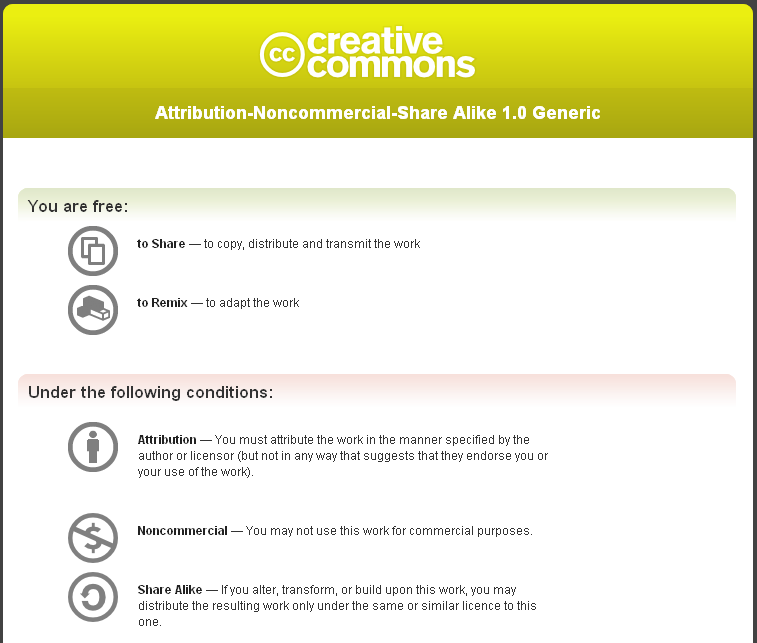
\includegraphics[width=0.50\textwidth]
		{assets/pics/creative_common.png}
		\caption{\license.}
		\label{fig:testGambar}
	\end{figure}


	%-----------------------------------------------------------------------------%
	\section{Membuat Tabel}
	%-----------------------------------------------------------------------------%
	Seperti pada gambar, tabel juga dapat diberi label dan caption.
	Caption pada tabel terletak pada bagian atas tabel.
	Contoh tabel sederhana dapat dilihat pada \tab~\ref{tab:tab1}.

	\begin{table}
		\centering
		\caption{Contoh Tabel}
		\label{tab:tab1}
		\begin{tabular}{| l | c r |}
			\hline
			        & kol 1 & kol 2 \\
			\hline
			baris 1 & 1     & 2     \\
			baris 2 & 3     & 4     \\
			baris 3 & 5     & 6     \\
			jumlah  & 9     & 12    \\
			\hline
		\end{tabular}
	\end{table}

	Ada jenis tabel lain yang dapat dibuat dengan \latex~berikut
	beberapa diantaranya.
	Contoh-contoh ini bersumber dari
	\url{http://en.wikibooks.org/wiki/LaTeX/Tables}

	\begin{table}
		\centering
		\caption{An Example of Rows Spanning Multiple Columns}
		\label{row.spanning}
		\begin{tabular}{|l|l|*{6}{c|}}
			\hline % create horizontal line
			No & Name & \multicolumn{3}{|c|}{Week 1} & \multicolumn{3}{|c|}{Week 2}                 \\
			\cline{3-8} % create line from 3rd column till 8th column
			   &      & A                            & B                            & C & A & B & C \\
			\hline
			1  & Lala & 1                            & 2                            & 3 & 4 & 5 & 6 \\
			2  & Lili & 1                            & 2                            & 3 & 4 & 5 & 6 \\
			3  & Lulu & 1                            & 2                            & 3 & 4 & 5 & 6 \\
			\hline
		\end{tabular}
	\end{table}

	\begin{table}
		\centering
		\caption{An Example of Columns Spanning Multiple Rows}
		\label{column.spanning}
		\begin{tabular}{|l|c|l|}
			\hline
			Percobaan               & Iterasi & Waktu    \\
			\hline
			Pertama                 & 1       & 0.1 sec  \\ \hline
			\multirow{2}{*}{Kedua}  & 1       & 0.1 sec  \\
			                        & 3       & 0.15 sec \\
			\hline
			\multirow{3}{*}{Ketiga} & 1       & 0.09 sec \\
			                        & 2       & 0.16 sec \\
			                        & 3       & 0.21 sec \\
			\hline
		\end{tabular}
	\end{table}

	\begin{table}
		\centering
		\caption{An Example of Spanning in Both Directions Simultaneously}
		\label{mix.spanning}
		\begin{tabular}{cc|c|c|c|c|}
			\cline{3-6}
			                                                &     & \multicolumn{4}{|c|}{Title}                 \\ \cline{3-6}
			                                                &     & A                           & B   & C   & D \\ \hline
			\multicolumn{1}{|c|}{\multirow{2}{*}{Type}}     &
			\multicolumn{1}{|c|}{X}                         & 1   & 2                           & 3   & 4       \\ \cline{2-6}
			\multicolumn{1}{|c|}{}                          &
			\multicolumn{1}{|c|}{Y}                         & 0.5 & 1.0                         & 1.5 & 2.0     \\ \cline{1-6}
			\multicolumn{1}{|c|}{\multirow{2}{*}{Resource}} &
			\multicolumn{1}{|c|}{I}                         & 10  & 20                          & 30  & 40      \\ \cline{2-6}
			\multicolumn{1}{|c|}{}                          &
			\multicolumn{1}{|c|}{J}                         & 5   & 10                          & 15  & 20      \\ \cline{1-6}
		\end{tabular}
	\end{table}
\fi


